\documentclass[conference]{IEEEtran}
\ifCLASSINFOpdf
\else
\fi
\usepackage[pdftex]{graphicx}
%\usepackage{tikz}
\usepackage{float}
\usepackage{array}
\usepackage{tabularx,booktabs}

\usepackage{amsmath} %Import AMS math package
\graphicspath{{/C:/Users/Jace/Desktop/3학년1학기/소프트웨어공학/Healpers/latex/}}
\DeclareGraphicsExtensions{.pdf,.png,.jpg,.jpeg}
\hyphenation{op-tical net-works semi-conduc-tor}
\begin{document}
\normalsize
\title{Self-Orthotherapy program\\ 
using Arduino and pressure sensor 
}

\author{\IEEEauthorblockN{Hakjun Kim}
\IEEEauthorblockA{Information System in HYU\\
Email: canon3478@gmail.com }
\and
\IEEEauthorblockN{Minsoo Choi}
\IEEEauthorblockA{Information System in HYU \\
Email: choiza03@gmail.com\\\\\Large{Group Name : 'Healpers'}}
\and
\IEEEauthorblockN{Taejin Kim\\Information System in HYU\\
Email: o\_\_\_xo@naver.com \\\\\\\\\\\\}}
\maketitle

\begin{abstract}

This project is about self-orthotherapy system using Arduino with a built-in bluetooth 4.0 communication chip and pressure sensor which communicates with an Android application. This program can definitely detect users' incorrect postures and can be used for long-term postural analysis and correction as saving users' postural data in database.\\

\emph{Keywords}---Self-orthotherapy, Arduino, Pressure sensor, Android application \\\\\\\\\\

\end{abstract}
\renewcommand{\arrayrulewidth}{1pt}


\begin{table}

\begin{tabular}{|c|c|l|}\hline

Role & Name & Task description and etc. \\ \hline \hline

&  &  -- Test the application in various postures. \\ 

User & Minsoo & -- Require bugs to be fixed.  \\ 

& Choi & -- Demand the all of data about user. \\ 

&  & -- Require additional functions. \\ \hline

&  &  -- Develop the application using Arduino and\\ 

Software & Taejin & pressure sensor. \\ 

Developer & Kim & -- Fix bugs. \\ 

&  & -- Develop additional functions according to\\ 

&  & users' needs. \\ \hline

&  &  -- Monitor the progress of the project. \\ 

Development & Hakjun & -- Make a overall plan about developing \\ 

Manager& Kim & program and managing the budget \\ 

&  & -- Reflect users' needs \\ \hline

\end{tabular}

\end{table}


\IEEEpeerreviewmaketitle
\large


\section{Introduction}

% no \IEEEPARstart
In modern society, most office workers spend over 12 hours each day sitting on a chair. This immoderate sedentary lifestyles and incorrect posture can cause many severe health problems. For instance, incorrect posture can lead to turtle neck syndrome, scoliosis, chronic low back pain, cervical disc and herniated disc. In particular, crossing legs can twist the pelvis which induces pelvis inflammation and may change the shape of spine and trigger crooked legs, all of which are the reason for an asymmetrical body. In other words, correct posture will be the most effective way to prevent the above diseases.

Therefore, maintaining a good posture in a forced sedentary lifestyle has a great significance to keep them healthy. Nevertheless, when office workers concentrate on working or loosen the tension, posture would be disturbed. So we would like to develop an application to help them correct their wrong postures.

The application can recognize the position by using Arduino and pressure sensor. The application will perform the correction of posture immediately by informing the users' incorrect postures. This application is expected to greatly contribute to maintaining a healthy posture and lifestyle of the modern office workers. 
\\\\\\
% You must have at least 2 lines in the paragraph with the drop letter
% (should never be an issue)

\section{Requirements}

\subsection{Required hardware and software}

-Arduino Uno R3 Board

-FSR 406(Pressure sensor)

-Connecting pin

-Bread Board

-HC 06(Bluetooth Module)

-USB cable

-Arduino Sketch(Using C)

-Android Studio(Using Java)

-MySQL\\


\subsection{Requirements for Developers}

-- Making pressure recognizing cushion

First, we have to make proper pressure recognizing cushion to recognize users' posture. So, we are going to make cushion with pressure sensors fitted to the chair's size. Now, we have plan to use 'FSR 406(Pressure sensor)' that the size is approximately 38mm x 38mm. So, we are going to make cushion with four(2x2) pressure sensors or more to recognize users' posture properly.   \\

-- Connecting  pressure sensor with Arduino Board

Second, we have to connect pressure sensor with Arduino Board to get pressure value. And we have plan to use 'Arduino Uno R3 board'. So, we are going to connect 'FSR pressure sensor' with 'Arduino Uno R3 board' and test whether we get proper pressure value when user changes the posture. \\

-- Making orthotherapy algorithm using pressure value

If we succeeded in getting proper pressure value, we make our own orthotherapy algorithm. We will analyze pressure values and set cases to correct users' posture. For example, when the right side's pressure value is low we show alert message (''Your body is tilted to the left'' or ''Don't let your right leg crossed''). \\

-- Developing  Front-end Android Application

After we make orthotherapy algorithm we have to develop 
android application. So, we will develop the application according to our UI/UX and architecture design. We have two parts in our front-end application. The first is the Self-Orthotherapy part and the second is showing analyzed result using users' personal data.\\

-- Constituting Database for saving users' data

We should design database tables for saving users' data.
And we make sign-up form for user to register in our application. And we get essential data such as ID, PW, Phone number and put it into the our database. \\

-- Developing  Server to manage users' data

We will provide analyzing service using users' personal data. So, we have to manage users' own Id and Password by server and save the users' specific data. For example, if the user got some alert messages or moves out the users' seat, we save that data and we will provide graph or chart by analyzing that data.\\

\subsection{Requirements for Users}
-- Getting alert message when having bad posture

If user had bad posture, program recognizes that and shows the alert message to fix that posture.  Bad posture means i) sit with one's legs crossed. ii) the waist is bended iii) the body is tilted to right or left too much.\\

-- Approaching users' personal data

User needs authority to approach to own personal data. So, user should sign-up for our application. After that, user could check own personal data any time. For instance, how many times the user sit with right leg crossed today or how long the user left the seat during the work concentration time.\\

\subsection{Requirements for Application}
-- Sign Up

This application uses the ID to the user by storing the time information of the server to be able to store and view the information, if not the own device. The user can easily sign up only your name, E-mail, if you ever forget your ID and Password can be easily found via E-mail.\\

-- Log In / Out

When running this application, user has to log-in in order to record the time sitting on the cushion on a server. But, to shorten the log-in procedure, user can log-in easily after log- in once because the information of ID and password is saved. If the User wants to log-out, user can logs out in the Setting Page.\\

-- Statistics

The application stores the users' data on the server. The application stores the users' data on the server. Then this application produces statistics on a weekly, monthly, yearly. These statistics will help determine whether seeing how much work they have kept for themselves some attitude.\\

-- Data Visualization

User allows to easily identify their own data through the application using the data visualization. The application will use the visualization techniques, such as Android Chrono-meter, Chart, VideoView.\\

-- Guide to Good Posture

This application shows the right postures using some kind of videos and images and introduces stretching and exercises which are good to correct wrong posture.\\

-- Suggest to Rest

If user overworks, this application will show the message likewise ''Take a Break! Do strectch!''.\\

-- Push Alarm

If user keeps wrong posture over certain time, this application will warn to the user about that wrong posture by push alarm.\\

-- Customize Setting

User can set the status of getting push alarm(On/Off) and the time when the user gets push alarm while the user keeps wrong posture. And the user could use ''Initializing'' function. ''Initializing'' means the user's own pressure values saved in the database (when user does 'normal' posture) are initialized.\\\\\\

-- Provide Scores

Users can grasp how well they have sat for today as this application provides today's posture score. Users can also check whether their postures are improving or not.

-- Body Balance Measurements

Users can measure their current body balance status by taking a photo of their upper body. If, users take picture by using this function, the program would offer the information about how much their body is twisted. 

\section{Development Environment}

\subsection{Choice of software development platform}

1. Which platform and why?  \\

-- Windows for android application developing

Our target is office workers who want to correct their sitting posture. For ortho-therapy, it is the most important and efficient to maintain correct posture intentionally. Considering this, developing mobile application is appropriate rather than either web or computer program operated in window OS because time with mobile phone is longer than time using computer. If there is only our posture-correcting cushion, users can notice that they sit in incorrect posture by push alarm at anytime and anywhere, even while watching TV and reading a book at home. And this data is saved in server automatically so they can check the statistics how long they were sitting and how many times they sat incorrectly. Because Android OS is being used much more than IOS, as the below Figure 1 is showing, we develop our application in Android application.

\begin{figure}[htbp]
\begin{center}
    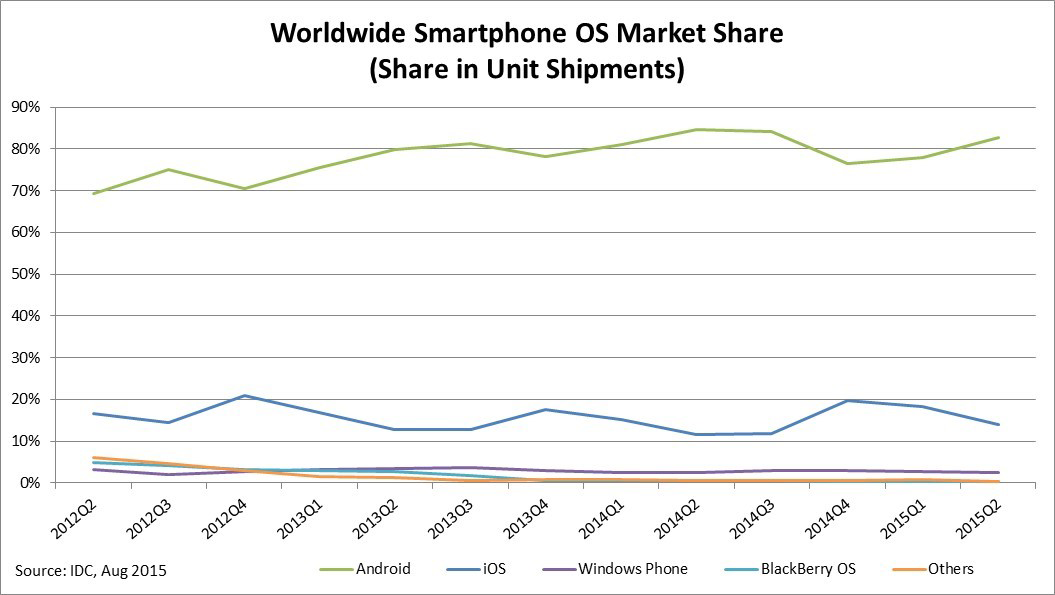
\includegraphics[scale=0.4]{img_03.png}
    \caption{Worldwide Smartphone OS Market Share} 
\end{center}
\end{figure}

2.	Which programming language and why?\\

-- Java for android application developing

Java is a general-purpose computer programming language that is concurrent, class-based, object-oriented, and specifically designed to have as few implementation dependencies as possible. As of now, Java is one of the most popular programming languages in use, particularly for client-server web applications, with a reported 9 million developers. Java was originally developed by James Gosling at Sun Microsystems (which has since been acquired by Oracle Corporation) and released in 1995 as a core component of Sun Microsystems' Java platform. The language derives much of its syntax from C and C++, but it has fewer low-level facilities than either of them. And Java is the best suitable language to develop the application in android OS.\\

-- C for IDE

We should do many tests to recognize various users' postures using pressure values getting from FSR-406 pressure sensors. So, we use the open-source Arduino Software (IDE) and the best proper language to use this program is C. The open-source Arduino Software (IDE) makes it easy to write code and upload it to the board. It runs on Windows, Mac OS X, and Linux. The environment is written in Java and based on Processing and other open-source software. This software can be used with any Arduino board.\\

-- PHP

PHP is a server-side scripting language designed for web development but also used as a general-purpose scripting language that is especially suited to web development. PHP is fast, flexible and pragmatic language. And PHP makes the user write dynamic web files because PHP follows many sentence forms used in C, Java, Perl etc. And there is excellent documentation we can refer to. http://www.php.net/ has really good documentation with helpful user-contributed gotchas and code snippets. We can also find tons of tutorials, etc. around the web.\\

3.	Provide a cost estimation for your built.\\

-- Cost for Server :

1 year for free. And after 1 year, there will be additional prices. We predict maybe about 1,000 people will use our service, and DAU (Daily Activity User) will be 300 around. So we will use t1. micro instance (AWS), and its prices are about 30 dollars per month: So may be there will be additional 360 dollars per year.\\

-- Cost for hardware

1)	Arduino

The Uno is a microcontroller board based on the ATmega328P. It has 14 digital input/output pins (of which 6 can be used as PWM outputs), 6 analog inputs, a 16 MHz quartz crystal, a USB connection, a power jack, an ICSP header and a reset button. It contains everything needed to support the microcontroller; simply connect it to a computer with a USB cable or power it with a AC-to-DC adapter or battery to get started. The Uno board and version 1.0 of Arduino Software (IDE) were the reference versions of Arduino, now evolved to newer releases. The Uno board is the first in a series of USB Arduino boards, and the reference model for the Arduino platform; for an extensive list of current, past or outdated boards see the Arduino index of boards.\\

2)	Pressure Sensors

The model 406 FSR is a single-zone Force Sensing Resistor optimized for use in human touch control of electronic devices such as automotive electronics, medical systems, and in industrial and robotics applications. FSRs are two-wire devices. They are robust polymer thick film (PTF) sensors that exhibit a decrease in resistance with increase in force applied to the surface of the sensor. It has a 39.6mm square active area and is available in 4 connection options. Interlink Electronics FSR 400 series is part of the single zone Force Sensing Resistor family.\\

3)	Bluetooth Module

HC-06 is a serial port module composed in SMD form which is possible to be replaced easily. It also uses the connection between the bluetooth Master module in either PC or mobile device and embedded system in substitution of the serial port. 

Arduino receives the input values, which the four pressure sensors perceive, through the breadboard and sends those values to the Android Application via bluetooth communication with the mobile phone. The system flow is shown in Figure 2.\\

\begin{figure}[H]
\begin{center}
    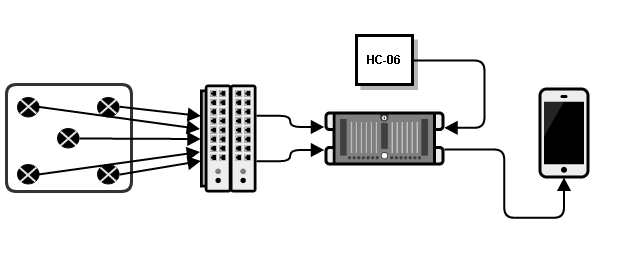
\includegraphics[scale=0.4]{img_01.png}
    \caption{System Flow} 
\end{center}
\end{figure}

Therefore, we need 4 pressure sensors, Arduino, bluetooth module, bread board, USB cable and jump wire MM. The specific products' cost is shown in Table 1.\\
\begin{center}

\begin{table}[H]
\caption{The Specific Products' Cost }
\begin{tabular}{|c|c|c|c|}\hline


Products & Prices & Quantities & Costs \\ \hline \hline

Pressure Sensor (FSR-406) & 14,000 & 4 & 56,000  \\ \hline 

Arduino Uno (R3) & 7,500 & 1 & 7,500 \\ \hline

Bluetooth Module (HC-06) & 6,000 & 1  & 6,000 \\ \hline

Bread Board & 4,500 & 1 & 4,500 \\\hline

USB Cable & 500 & 1 & 500  \\ \hline

Jump Wire MM& 70 & 50 & 3500  \\ \hline

\multicolumn{3}{|c|}{Total} & \multicolumn{1}{|l|}{78,000} \\ \hline 

\end{tabular}
\end{table}
\end{center}

4.	Provide clear information of your development environment. (e.g., version of software, OS version, your computer resources)\\

-	Android develop

1)	Windows : Windows 10

2)	Android Studio 1.5.1 / Android 4.4.4 Kitkat\\

-	Arduino develop 

3)	Windows : Windows 10

4)	Arduino 1.6.8 (IDE)\\


5.	Using any commercial cloud platform (e.g., Amazons EC2) is definitely a BONUS.\\

 We will use Apache Web Server because it is the world's most widely used web server software. As of June 2013, Apache was estimated to serve 54.2 percent of all active website and 53.3 percent of the top servers across all domains. (The most important reason is we have already apache web server.)\\

Apache Web Server has some features:

- easy and fast customizing using module.

- It can handle many traffic easily.

- It can control web server more delicately

- It is tested enough, so it is very stable.\\

\subsection{Software in use}

-	Footlogger

3L-Labs, internal venture corporation, developed a smart wearable device 'FootLogger'. It is insoles with some pressure sensors which analyze users' steps. This device can be used for health care, sports and entertainment.\\

Healthcare

- Monitors recovery after surgery

- Assesses balance of diabetics

- Allows for monitoring of prescribed exercises 

- Monitors safety and activity of senior citizens

- Activity tracking (calories, distance, time)

- Early prediction of dementia and spinal disease

- Early prediction of accidents from falling

- Monitors rehabilitation (stroke, paralysis)\\

Sports

- Can monitor distance traveled

- Monitors golf stance and gives coaching

- Marathon/jogging aid

- Out-toeing/in-toeing gait identification, provides 

gait coaching
 
- Kids' correct posture coaching

- Can be applied to every sport\\

Entertainment

-  Daily log (standing, sitting, walking)

-  Personality analysis

-  Daily mood analysis

-  Smartphone game input device\\

\begin{figure}[H]
\begin{center}
    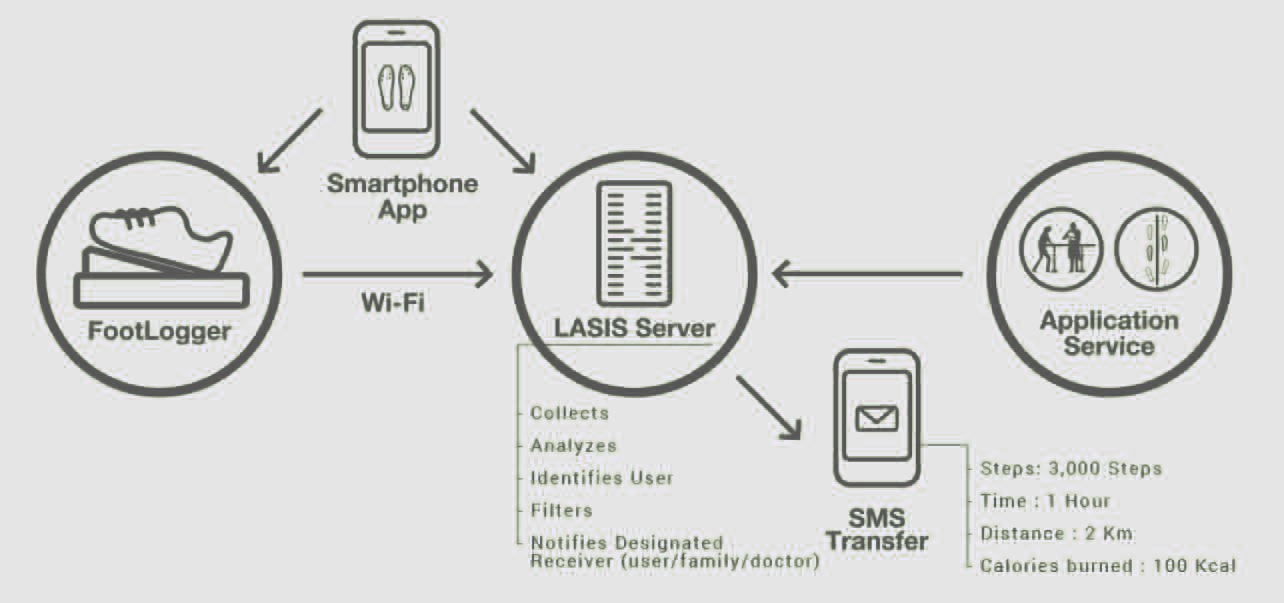
\includegraphics[scale=0.33]{img_05.jpg}
    \caption{Footlogger} 
\end{center}
\end{figure}

\subsection{Task distribution}

\renewcommand{\arrayrulewidth}{1pt}


\begin{table}[H]
\caption{task distribution}
\begin{tabular}{|c|c|l|}\hline
Role & Name & Task description and etc.\\ \hline \hline

&  &  -- Test the application in various postures. \\ 

User & Minsoo & -- Require bugs to be fixed.  \\ 

& Choi & -- Demand the all of data about user. \\ 

&  & -- Require additional functions. \\ \hline

&  &  -- Develop the application using Arduino and\\ 

Software & Taejin & pressure sensor. \\ 

Developer & Kim & -- Fix bugs. \\ 

&  & -- Develop additional functions according to\\ 

&  & users' needs. \\ \hline

&  &  -- Monitor the progress of the project. \\ 

Development & Hakjun & -- Make a overall plan about developing \\ 

Manager& Kim & program and managing the budget \\ 

&  & -- Reflect users' needs \\ \hline

\end{tabular}\\\\\\\\

\end{table}

\section{Specifications}

\subsection{Modeling for Specifications \\}


\begin{figure}[H]
\begin{center}
    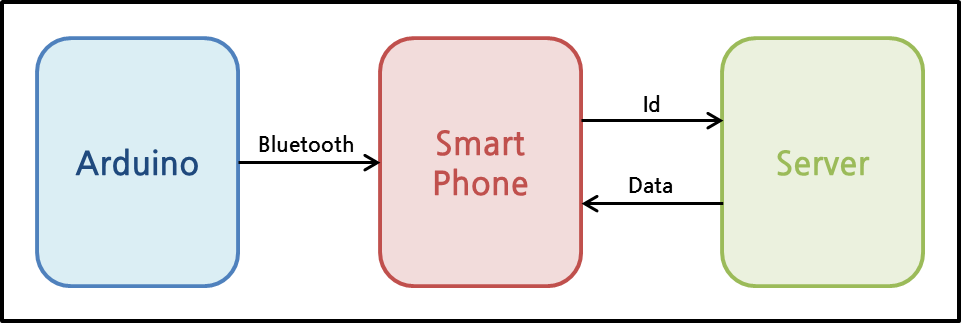
\includegraphics[scale=0.55]{img_04.png}
    \caption{Basic structure} 
\end{center}
\end{figure}


 Arduino receives some of the pressure value from the pressure sensor. And arduino sends the values to smart phone using HC-06. HC-06 is a Bluetooth Module. Then smart phone application determines posture of the user by analyzing the values. After that, smart phone calculates the time for holding the posture. The data of time will be sent to server, and saved at server.
At the same time, the application will receive the user's whole data from server. Then, the application will display the data by data visualization.\\\\

\subsection{Posture Recognition using pressure sensor}
 We made a kind of cushion for measuring pressure force. The dimensions of the chair and cushion are shown in Table 3. And we used FSR-406 pressure sensor model to get proper pressure value for recognizing person's changing posture. The dimensions of FSR-406 are shown in Figure 5.\\
 
 \begin{table}[h]
{\renewcommand\arraystretch{1.25}
\caption{Dimensions of the chair and cushion}
\begin{tabular}{|c|cc}  \hline\hline
Width of the chair& \multicolumn{2}{p{5cm}|}{\raggedright 45cm} \\ \hline
Height of the chair& \multicolumn{2}{p{5cm}|}{\raggedright 42cm} \\ \hline
Depth of the chair& \multicolumn{2}{p{5cm}|}{\raggedright 47cm} \\ \hline
Width of the cushion& \multicolumn{2}{p{5cm}|}{\raggedright 30cm} \\ \hline
Height of the cushion& \multicolumn{2}{p{5cm}|}{\raggedright 30cm} \\ \hline \hline
\end{tabular}}
\end{table}


\begin{figure}[H]
\begin{center}
    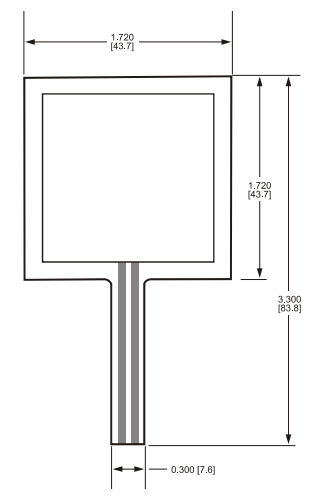
\includegraphics[scale=0.6]{img_06.png}
    \caption{Dimensions of FSR-406} 
\end{center}
\end{figure}

The reason why we choose the FSR-406 is the specifications of FSR-406 are suitable to make the posture recognition cushion. This sensor is very thin and hence can be easily bent to fit, so a user can sit down on the seat comfortably. Since the sensor sheet is light and thin, it can be carried anywhere and used in various situations in daily life. And the active area is appropriate to get pressure value when person changes his or her posture. FSR-406 specifications are shown in Table 4.

 \begin{table}[h]
{\renewcommand\arraystretch{1.25}
\caption{FSR-406 specifications}
\begin{tabular}{|c|cc}  \hline\hline
Thickness& \multicolumn{2}{p{6cm}|}{\raggedright 0.018'' (0.46 mm)} \\ \hline
Active area& \multicolumn{2}{p{6cm}|}{\raggedright 38.1mm $x$ 38.1mm} \\ \hline
Connector& \multicolumn{2}{p{6cm}|}{\raggedright AMP Female connector} \\ \hline
Minimum load& \multicolumn{2}{p{6cm}|}{\raggedright 0.1N} \\ \hline
Maximum load& \multicolumn{2}{p{6cm}|}{\raggedright 10N} \\ \hline \hline
\end{tabular}}
\end{table}



FSRs are two-wire devices with a resistance that depends on applied force. For specific application needs please contact Interlink Electronics support team. An integration guide is also available. For a simple force-to-voltage conversion, the FSR device is tied to a measuring resistor in a voltage divider configuration. The output is described by the equation:


\begin{displaymath}
\qquad\mathrm{V}_{out} =\frac{{R}_mV+}{({R}_M+{R}_{FSR})}\\
\end{displaymath}

In the shown configuration, the output voltage increases with increasing force. If ${R}_{FSR}$ and ${R}_{M}$ are swapped, the output swing will decrease with increasing force. These two output forms are mirror images about the line ${V}_{out}$  = $(V+) / 2$. The measuring resistor, ${R}_{M'}$ is chosen to maximize the desired force sensitivity range and to limit current. Depending on the impedance requirements of the measuring circuit, the voltage divider could be followed by an on-amp. A family of FORCE vs. ${V}_{out}$ curves is shown on the graph above for a standard FSR in a voltage divider configuration with various ${R}_{M}$ resistors. A $(V+)$ of $+5V$ was used for these examples.

\begin{figure}[htbp]
\begin{center}
    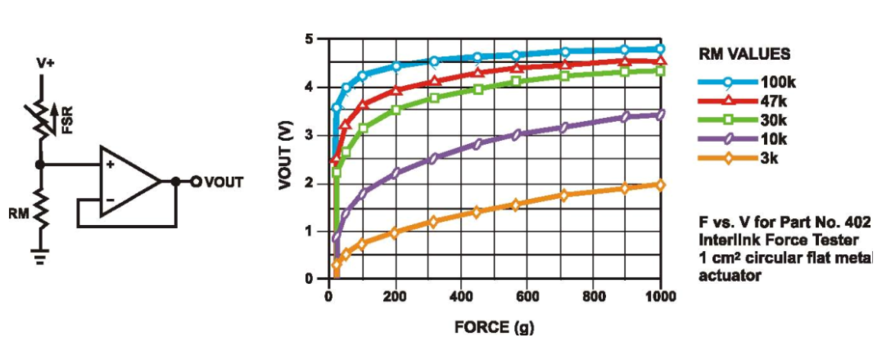
\includegraphics[scale=0.375]{img_07.png}
    \caption{Typical Schematic and force curve of FSR-406} 
\end{center}
\end{figure}

To recognize difference of sitting posture, we have to make the cushion with proper number of pressure sensors. So, we arranged five pressure sensors to the five points in the cushion. The five points are 'Left-front', 'Right-front', 'Center', 'Left-back', 'Right-back' and this classification is shown in Table 5. And the pressure values are transmitted to Arduino board through bread board. The pressure sensors' spot position is shown in Figure 7.

 \begin{table}[h]
{\renewcommand\arraystretch{1.25}
\caption{The classification of pressure sensor's position}
\begin{tabular}{|c|cc}  \hline\hline
(LF)& \multicolumn{2}{p{7cm}|}{\raggedright Left Front} \\ \hline
(RF)& \multicolumn{2}{p{7cm}|}{\raggedright Right Front} \\ \hline
(C)& \multicolumn{2}{p{7cm}|}{\raggedright Center} \\ \hline
(LB)& \multicolumn{2}{p{7cm}|}{\raggedright Left Back} \\ \hline
(RB)& \multicolumn{2}{p{7cm}|}{\raggedright Right Back} \\ \hline \hline
\end{tabular}}
\end{table}


\begin{figure}[H]
\begin{center}
    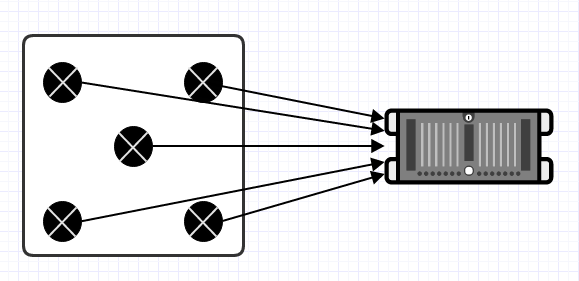
\includegraphics[scale=0.5]{img_08.png}
    \caption{Pressure sensors' spot position} 
\end{center}
\end{figure}

\subsection{Posture classification\\}

In this part, we describe a way of classifying sitting postures. Posture classification involves three basic issues. One issue is person dependency. Different persons would obviously sit in different ways. Even the same person might sit on different parts of the seating face. One ways to resolve this problem is to normalize pressure distributions by standardizing different postures when workers sit in the chair. The classification of seven postures is shown in Table 6.

 \begin{table}[h]
{\renewcommand\arraystretch{1.25}
\caption{The classification of seven postures}
\begin{tabular}{|c|cc}  \hline\hline
(N)& \multicolumn{2}{p{7cm}|}{\raggedright Left Front} \\ \hline
(F)& \multicolumn{2}{p{7cm}|}{\raggedright Leaning Forward} \\ \hline
(B)& \multicolumn{2}{p{7cm}|}{\raggedright Leaning Backward} \\ \hline
(L)& \multicolumn{2}{p{7cm}|}{\raggedright Leaning Left} \\ \hline
(LC)& \multicolumn{2}{p{7cm}|}{\raggedright Left leg crossed} \\ \hline 
(R)& \multicolumn{2}{p{7cm}|}{\raggedright Leaning Right} \\ \hline
(RC)& \multicolumn{2}{p{7cm}|}{\raggedright Right leg crossed} \\ \hline \hline
\end{tabular}}
\end{table}



Second issue is the time dependency. We have to push alarm to users when they are doing wrong postures. So, it is needed to decide when we do alarm function. We set time standard from 1 minute to 10 minutes. User could select time when user gets push alarms while user keeps wrong posture. 
   And the last issue is weight dependency. The sensor values would increase linearly or non-linearly with an increase in weight. Therefore, it would be effective to divide the sensor values by the total value. And the each user's pressure value is different when user does 'Normal' posture. So, if user registers in our application, the user's initial pressure values are saved in the database and our algorithm uses each user's data to recognize posture. And we offer the function which initializes user's weight in the application. 
\subsection{Specification for Bluetooth communication}

We use Arduino board and bluetooth module to get pressure values in the application and do wireless communication. There are many ways doing wireless communication with Arduino such as Wifi, XBee, Bluetooth etc. But Wifi wastes electronic power consuming too much and the connection status is sometimes not stable. And XBee is not widely used because smart phone and pc should have XBee module. On the other hand, Bluetooth module is cheaper than Wifi module and is widely used compared to Xbee because most of the smart phone and pc could recognize bluetooth module. And we use 'Arduino Uno R3' and 'HC-06' because 'Arduino Uno R3' is the basic platform among arduino series and 'HC-06' bluetooth module has excellent performance compared with other bluetooth modules and both of them have very good cost-effectiveness. And bluetooth sets the link with 'Master' and 'Slave' way. If mobile application communicates with arduino bluetooth, the smart phone becomes 'Master' and Arduino becomes 'Slave'. So, we connect HC-06 with Arduino Uno R3, this is shown in Figure 8.

\begin{figure}[h]
\begin{center}
    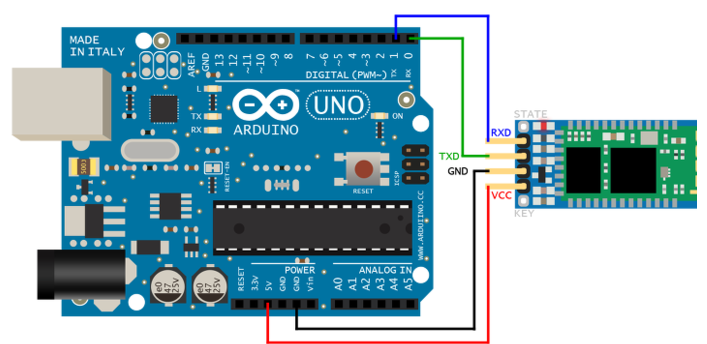
\includegraphics[scale=0.45]{img_02}
    \caption{Connection of arduino with bluetooth module} 
\end{center}
\end{figure}

The 'Blue' line is connection RX pin of HC-06 with digital I/O number 2 of Arduino (RX pin gets some signal from Arduino). The 'Green' line is connection TX pin of HC-06 with digital I/O number 3 of Arduino (TX pin transmits some signal from bluetooth). The 'Black' line is connection GND pin of HC-06 with GND of Arduino (GND is a voltage emitter). The 'Red' line is connection VCC pin of HC-06 with 5V of Arduino (VCC is a votage collector). 

And we set HC-06's options to test status of connection with bluetooth and pc. The sample option values of HC-06 are shown in below box.\\

\fbox{
  \parbox{0.42\textwidth}{
    1. Test
   Instruction word: AT 
   Return Value: OK\\
 
2. Version Checking
   Instruction word: AT+VERSION
   Return Value: OKlinvorV1.8 \\

3. Name Change
   Instruction word: AT+NAME
   Return Value : OKsetname\\

4. Baud rate Setting
    Instruction word: AT+BAUD(Baud rate menu value).
    Baud rate menu:
     1 - 1200,  2 - 2400, 3 - 4800,  4 - 9600
     5 - 19200,  6 - 38400, 7 - 57600,  8 - 115200 
    Return Value : OK Baud rate (ex : OK9600)\\

5. PIN Setting
   Instruction word: AT+PIN(4 digits).
   Return Value
 : OKsetPIN
  }
}

\subsection{Specification for front-end application pages\\}



 --	Log-In Page\\

\begin{figure}[h]
\begin{center}
    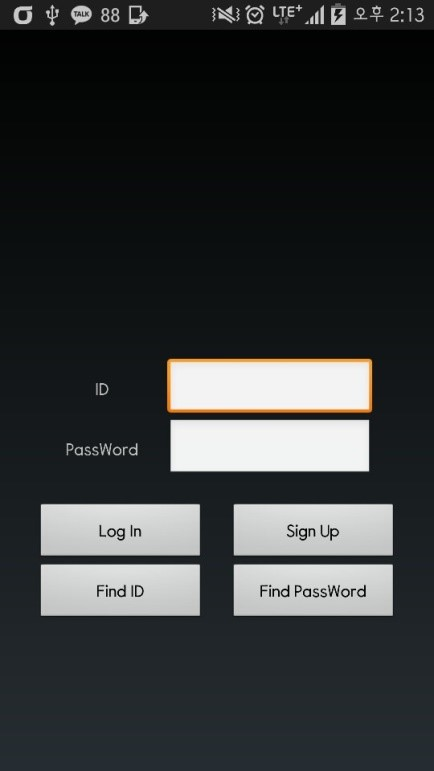
\includegraphics[scale=1]{img_10}
    \caption{Log-In Page} 
\end{center}
\end{figure}

 This page is the first page of the application. To import the posture data, you have to log in first. Your working posture records will be saved in your server with your ID. If you do not have an ID, you can click the Sing Up  button. Or, if you forgot your ID or password, you can find it using Find ID button or Find Password button. Once you log in, your ID and password will be automatically saved. Even when you log in via another phone, you can  open your records with ease since your posture records are imported from your ID only.\\

 -- Sign-Up Page\\
 
\begin{figure}[h]
\begin{center}
    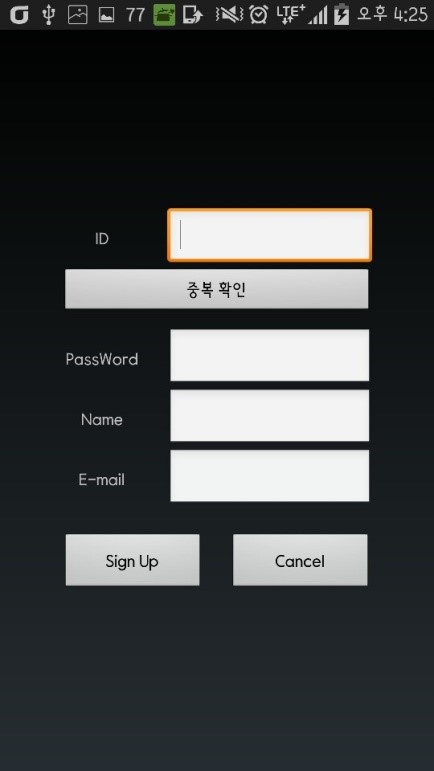
\includegraphics[scale=1]{img_11}
    \caption{Sign-Up Page} 
\end{center}
\end{figure}

 This page is where a user with no ID can create a new ID. Since ID will be the Primary Key of the User DB that will be saved in the server, it should not be overlapped. So, it is mandatory for you to double-check your ID. There is  no limit in the length of the password and the password will be replaced with other letters, such as ****, as soon as you enter your password for the sake of absolute confidentiality.

 Name and E-mail will be used for discerning between members and non-members. And, they will also be used for finding ID or Password in case you forgot it.\\

 -- Find ID Page\\

 Once you enter your E-mail that you entered during Sign-up process, it tells your ID on the screen.\\

 --Find Password Page\\

 Once you enter your E-mail that you entered during Sign-up process, it sends your password to your E-mail.\\
 
 --Now Page
 
\begin{figure}[h]
\begin{center}
    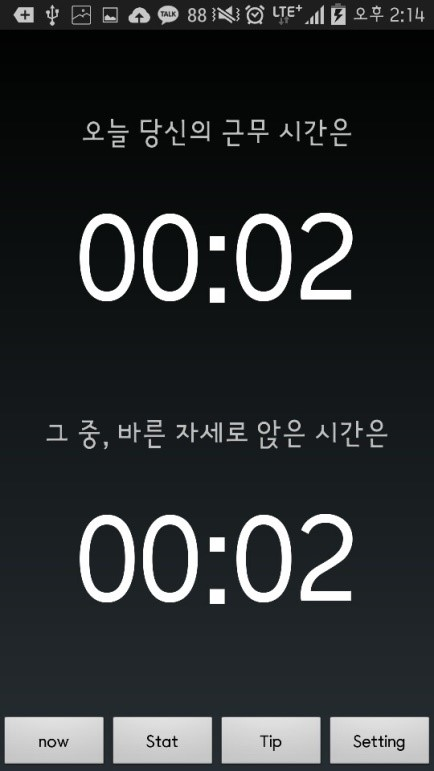
\includegraphics[scale=1]{img_12}
    \caption{Now Page} 
\end{center}
\end{figure}

 This page is the first page you see after you log in. There are 4 tabs in the tab bar below. 'Now' tab is the tab of the current page. If you click the 'Stat' tab, you can check your accumulated statistics on daily, weekly, monthly  and yearly basis. 'Tip' tab is where you can find images and videos of stretches or exercises useful for correcting posture. The last 'Setting' tab is for setting few functions related to this application.

 In this page, the app counts the number of hours you sit on the cushion that is composed of pressure sensor. This data will be exported on the screen in order for you to check your total working hour. (Upper Timer)
 
In specific, it counts the number of hours of your correct posture and bad posture separately. So, it is possible to check the number of hours of correct posture only. (Lower Timer)

 The number of hours exported from this page will be saved in the server as well. Moreover, once the user maintains a bad posture for a long time, the user will receive a push notification that warns his/her long-time bad  posture.\\

 --Stat Page

\begin{figure}[h]
\begin{center}
    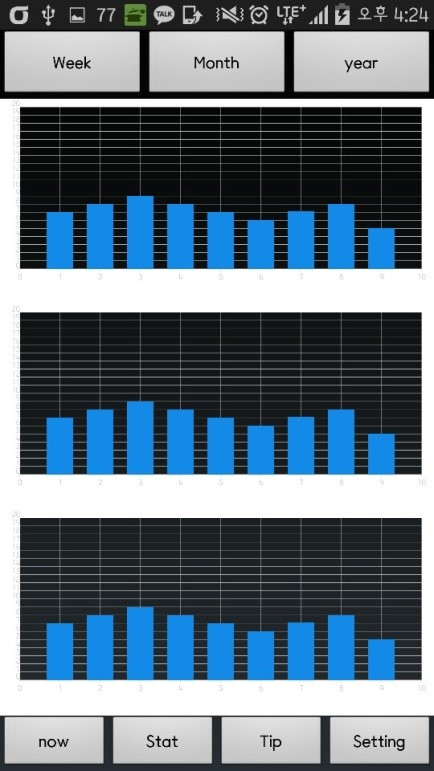
\includegraphics[scale=1]{img_13}
    \caption{Stat Page} 
\end{center}
\end{figure}

This page shows up as you click the Stat tab below. It is divided into 3 big graphs and has three tabs at the top of the screen. The graphs of this page are composed of individual time data saved in the server. Each of the  three graphs represents total working hour, the number of hours of correct posture and the bad posture.
The x-axis of this graph changes according to the upper tab of the screen. The x-axis consists of 7 days in the 'Weekly' tab, 30 days in the 'Monthly' tab and 12 months in the 'Yearly' tab.
The y-axis of every tab consists of numbers from 0 to 24, which refer to the number of hours.

 The first graph will be presented as a Bar Chart that shows working hour of the days of the week in the 'Weekly' tab, daily working hour in the 'Monthly' tab and monthly average working hour in the 'Yearly' tab.
With the same principle, the second graph shows the number of hours of correct posture for each tab whereas the third graph shows the number of hours of the bad posture.

And user could see the score measuring by this program. The score means how well users have sat for today. The score is from 0 to 100 and 100 is the maximum score which means the users posture for today is perfect.\\

 --Tip Page

\begin{figure}[htbp]
\begin{center}
    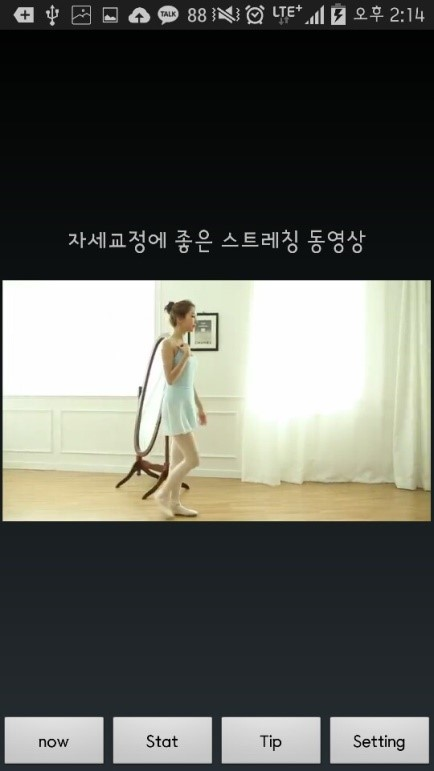
\includegraphics[scale=1]{img_14}
    \caption{Tip Page} 
\end{center}
\end{figure}

When clicking the Tip tab below this page, this page will show up. It exports images and videos of stretches or exercises useful for correcting posture as a customized ListView. The function of playing or pausing the video takes the similar format with Youtube. The first click plays the video and the second pauses it.\\

 --Setting Page

\begin{figure}[htbp]
\begin{center}
    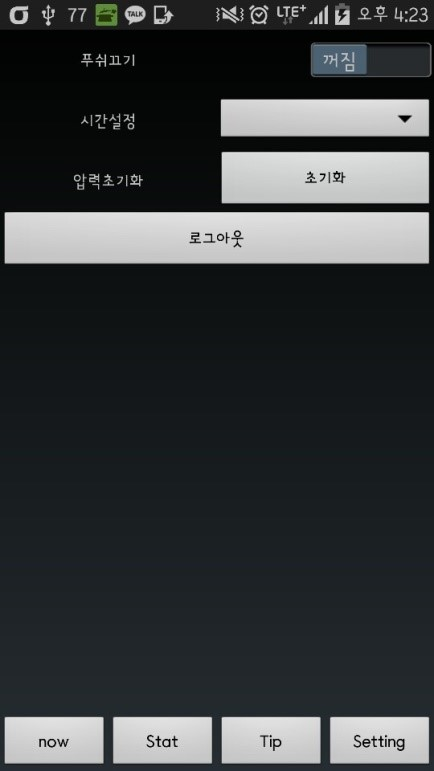
\includegraphics[scale=1]{img_15}
    \caption{Setting Page} 
\end{center}
\end{figure}

This page shows up when you click the 'Setting' tab below this page. The first function of this page, comprised of a ListView, is switching on or off the push notification. Essentially, if the user maintains a bad posture for a long time, the user will receive a push notification that warns his/her long-time bad posture. This function can be controlled by the user. 

The second function is to set the time when user gets push alarms while user keeps wrong posture. It ranges from minimum 1 minute to maximum 10 minutes. For example, if you set your time to 2 minutes and you maintain a bad posture for 2 minutes, you will directly receive a notification.

The third function resets the pressure value that matches the users' body. According to individuals' weight and environment, the pressure value differs. Hence, it is necessary to save individuals' initial pressure value of the  correct posture in the server. The last but not least function is log-out. It allows the user to log out from the app.\\

 -- Body Balance Page 
 In this page users could take picture of their upper body sitting on the chair. And the program analyses the users body balance by comparing left and right location of shoulder, chest and waist. Then the program shows how much the users body is twisted using degree. For example if the user's left shoulder is tilted to the left about 30 degrees, the user could see the status of the body balance by green and red line(Green line is criteria line meaning good body balance and the Red line shows how much the body is tilted.)and the message like ''Your left shoulder is tilted to the left about 30 degrees'' is shown. 
\\\\\\

\section{architecture design and implementation\\}

\subsection{Overall architecture}

\begin{figure}[H]
\begin{center}
    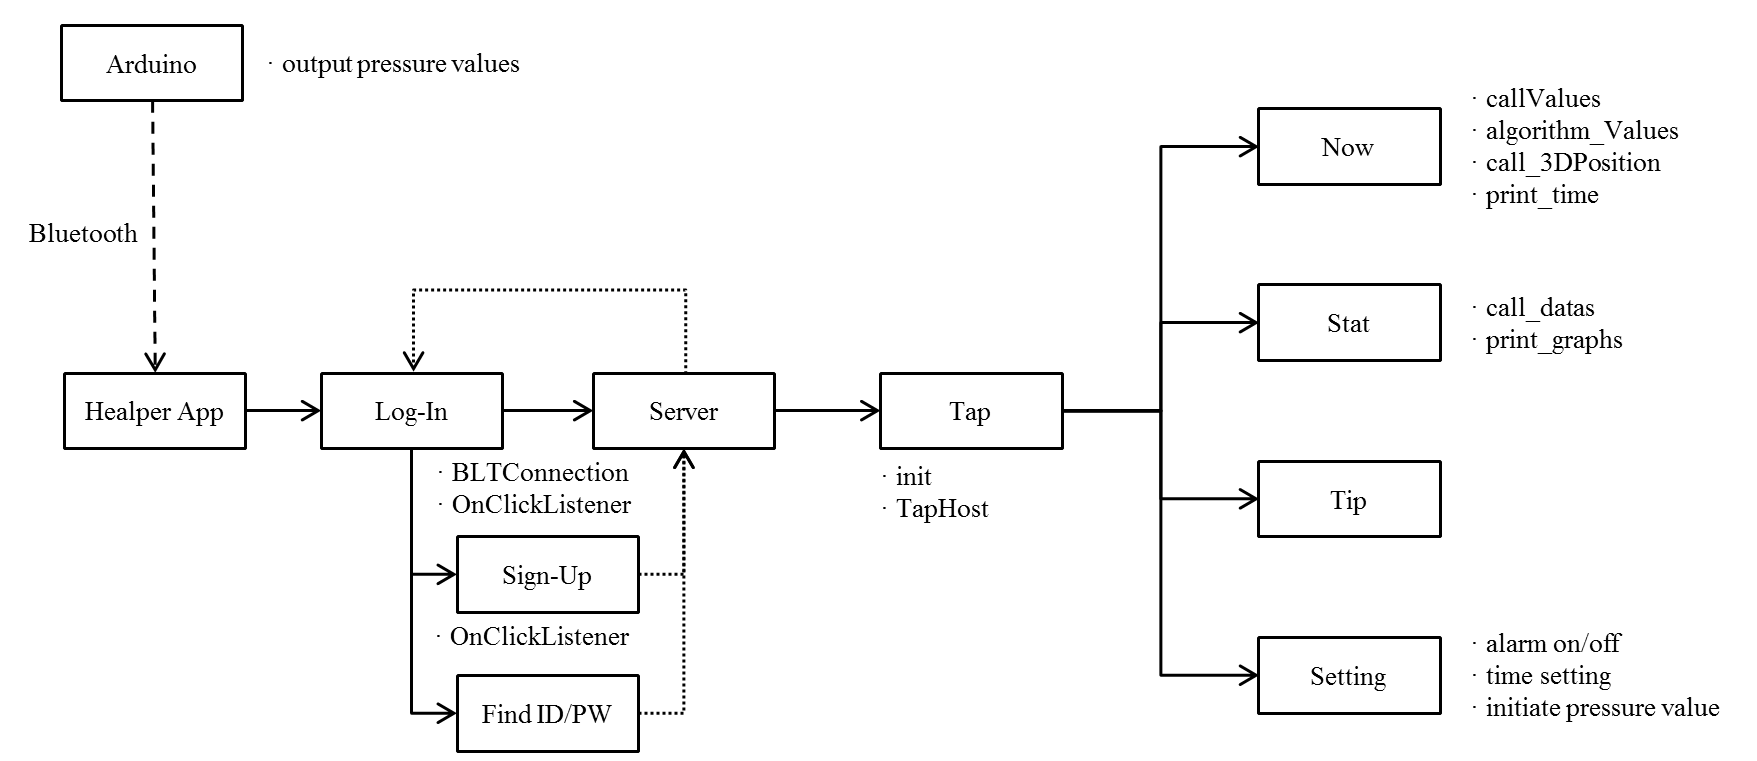
\includegraphics[scale=0.24]{img_16}
    \caption{overall architecture} 
\end{center}
\end{figure}

\subsection{Directory organization}

\begin{verbatim}
Dir 1: 
Healper_Proto/app/src/main/java/
com/example/lg/healper_proto

Dir 2:
Healper_Proto/app/src/main/res/
layout
\end{verbatim}

\begin{table}[H]
\caption{Directory Organization}
\begin{tabular}{|c|c|c|c|}\hline

Directory & File names & Module name in use & Etc \\ \hline \hline

Dir1 & MainActivity.java & MainActivity class & \\ \hline 

Dir1& NowActivity.java & NowAcivity class & \\ \hline 

Dir1 & SettingActivity.java & SettingActivity class & \\ \hline 

Dir1 & SignUpActivity.java & SignUpActivity class & \\  \hline 

Dir1 & StatActivity.java & StatActivity class & \\ \hline 

Dir1& TapActivity.java & StatActivity class & \\ \hline 

Dir1 & TipActivity.java & TipActivity class & \\ \hline 

In Arduino & ValuesToApp.ino & setup, loop method & \\ \hline  

Dir2& main\_{}sub.xml & & \\ \hline 

Dir2& now\_{}sub.xml & &  \\ \hline

Dir2& setting\_{}sub.xml & & \\ \hline 

Dir2 & signup\_{}sub.xml & & \\ \hline 

Dir2 & stat\_{}sub.xml & & \\ \hline 

Dir2 & tap\_{}sub.xml & & \\ \hline

Dir2 & tip\_{}sub.xml & & \\ \hline
\end{tabular}\\\\\\\\

\end{table}

\subsection{Code analysis\\}

1. ValuesToApp.ino\\

 -- Purpose: 

To send the pressure value that Arduino receive from the pressure sensor to the application through bluetooth,\\

 --	Functionality:

This code is embedded in the Arduino. The pressure sensor accepts the pressure value every second, and the pressure value is sent to the application through bluetooth. \\

 --	Location of source code:

In Arduino\\

 --	Class components:

a. Setup method 

Setup method is used firstly when the Arduino is executed. In this program, the speeds of serial communication and bluetooth communication are established in setup method. Variables and Pin value that is connected with the pressure sensors are declared and established. 

b. Loop method 

Loop method is used constantly while the Arduino is executed. In this program, the functions receiving and sending the pressure value are established in loop method. \\\\

2. MainActivity\\

 --	Purpose:
 
To show main page and before the program is used in earnest, to set fundamental environment.\\

 --	Functionality:
 
This program uses ID and password functions to save each user's individual data. For this, MainActivity provides log-in function that each users can log-in as their ID, sign-up function for users who start to use, find ID/password function for users who have forgotten theirs and bluetooth function for interworking specific cushion. \\

 -- Location of source code:
 
\begin{verbatim}
Healper_Proto/app/src/main/java/
com/example/lg/healper_proto/
MainActivity.java
\end{verbatim}

 -- Class components:

a. BLTConnection method

Relationship between the pressure sensors and smartphone is necessary because this program receives users’ posture data from the pressure sensor. In onClick method, BLTConnection method performs on/off functions and searching/connecting devices functions of bluetooth. Therefore, BLTConnection method is necessary in the first page, that is to say Log-In Page. 

b. OnClickListener

There are four OnClickListner in MainActivity.

  1) Log\_()In
  
When users enter their ID and password and click Log-in Button, if the account is signed up for server, loading data that are associated with the account from server synchronize with moving to TapActivity. Unless the account is signed up for server, Sign-Up Page appears.

  2) Sign\_()Up
  
Users who start to use this program use Sign-up button to sign up. When this button is clicked, Sign-Up Page appears.

  3) Find ID/ Find Password
  
When users have forgotten their ID or password, Find ID/Find Password button is used to move to Find ID/Password Page.\\\\

3.	SignUpActivity\\

 --	Purpose:

To show Sign-Up Page to users who start to use this program. Users can sign-up in Sign-Up Page. \\

 --	Functionality:

This activity saves new users' accounts information. In this activity, therefore, ID that is going to be the primary key goes through the duplication check and individual account information are saved in server.\\
 
 --	Location of source code:

\begin{verbatim} 
Healper_Proto/app/src/main/java/
com/example/lg/healper_proto/
SignUpActivity.java
 \end{verbatim}
 
 --	Class components:

a. OnClickListener

There are three OnClickListner in SignUpActivity.

  1) Redundancy\_()Check

  Individual account information reported in this page is going to be saved in server. Each user's ID is going to be the primary key in server database. Therefore, the duplication check is necessary to check if an entered ID that tries to sign-up is same as other existing users' ID. There are duplication check button for this. 

  2) Sign\_()Up

  Account information entered by users is saved in server and moves back to Log-In Page again.

  3) Cancel

  Cancel Sign-Up process moves back to Log-In Page again.\\\\



4.	TapActivity\\
 
 --	Purpose:
 
To show tap page and constitute tap view which consist of Now, Stat, Tip, and Setting for customer.\\
 
 --	Functionality:

TapActivity is the body of this program. We build this program to make users be able to transfer freely using 'tab' from a tap to another tap among four taps; now status, statistics, tips and setting page. TapActivity is used in this part to make Fragment Activity showing each page as fragment.\\

 --	Location of source code:
 
\begin{verbatim}
Healper_Proto/app/src/main/java/
com/example/lg/healper_proto/
TapActivity.java
 \end{verbatim}
 
 --	Class components:

a. Init method

Init method in onCreate method, when this page is created, initialize all of taps to interwork each other. 

b. TapHost

when four taps at the bottom of the page are clicked, Fragment is changed to an activity corresponding the tap. Switching page is convenient by using taps. \\\\

5.	NowActivity\\

 --	Purpose:

NowActivity shows users' current posture. It helps users grasp what posture and how long they have adopted.  \\

 --	Functionality:

NowActivity analyzes the pressure value that comes from Auduino through bluetooth. It also helps users see their current postures in 3D and shows how long the users have adopted the postures and how long they have sat by using chronometer function.\\

 --	Location of source code:
 
\begin{verbatim}
Healper_Proto/app/src/main/java/
com/example/lg/healper_proto/
NowActivity.java
\end{verbatim}

 --	Class components:

a. callValues method 

callValues method in onCreateView saves the pressure values that are sent from Arduino through bluetooth in variables to input those values in algorithm\_()Values. 

b. algorithm\_()Values method 

Using the pressure values saved in variables by callValues method, it outputs the anatomy-computed current posture by input the variables in designed algorithm for analogizing the current posture. 

c. call\_()3Dposition method 

call\_()3Dposition method invokes 3D\_()Position Graphic file corresponding current posture that is computed by algorithm\_()Values and displays it in Now Page. 

d. print\_()time method 

print\_()time method displays users' total sitting time and the time users have adopted their current postures in Now Page. \\\\


6.	StatActivity\\

 --Purpose:

StatActivity makes statistical charts of users' posture data in server and displays three graphs arranged by the week, the month and the year. \\

 --	Functionality:

StatActivity loads users' data from server, makes statistical charts and by three graphs, helps users grasp their posture tendencies that they have adopted. \\

 --	Location of source code:
 
\begin{verbatim}
Healper_Proto/app/src/main/java/
com/example/lg/healper_proto/
StatActivity.java
 \end{verbatim}
 
 --	Class components:
 
a. call\_()data method 

call\_()data method in onCreateView loads a recent year's data of users from server. That loaded data is saved in time\_()array.  

b. print\_()graphs method 

Using data that is saved in variables through call\_()datas method data, makes graphs and displays them in Stat Page.\\\\

7.	TipActivity\\

 --	Purpose:

To select and recommend orthotherapy videos that users probably need mostly after analyzing their postures. \\

 --	Functionality:

StatActivity analyzes today's posture statistics and recommend the orthotherapy exercise for the particularly bad posture in priority. On the basis of data of server, furthermore, it recommends two or three exercises for the steadily bad postures. \\

 --	Location of source code:
 
\begin{verbatim} 
Healper_Proto/app/src/main/java/
com/example/lg/healper_proto/
TipActivity.java
\end{verbatim}

 -- Class components\\\\
 
8.	SettingActivity\\

 --	Purpose:

To configure software setting and hardware setting to suit users' individual conditions. \\

 --	Functionality:

This program basically lets users know that they are maintaining bad posture by push alarm. However, it also has  function that turns on/off push alarm function for the case that users do not want to be disturbed by push alarm. Or users can configure schedule time when they want to be alarmed. Because every user has different weights and balances, in addition, we added reset function in Setting Page in case of that basic pressure value of postures might need to be configured newly. \\

 -- Location of source code:

\begin{verbatim}
Healper_Proto/app/src/main/java/
com/example/lg/healper_proto/
SettingActivity.java
\end{verbatim}

 --Class components:

a.	alarm on/off method

There is a on/off switch for the push alarm in Setting Page. As we established on/off function in onClickListener of this switch, users can choose whether they turn on the push alarm or not.

b. time setting method

There is a list box in Setting Page. In this list box, there are ten options; from 1 minute to 10 minutes. After that time user selects, push alarm informs that users are maintaining the bad postures.
 
c. initiate pressure value method

Setting up a common pressure value is impossible since every users have different pressure values. Therefore, we made it possible that every users configure their own pressures value. When initialization button in Setting Page is clicked, the average pressure value that has input for five seconds is saved in application and also in server. This program judges whether users' current postures are wrong or not comparing with the saved values. \\\\\\


\section{Use Cases}
\begin{figure}[H]
\begin{center}
    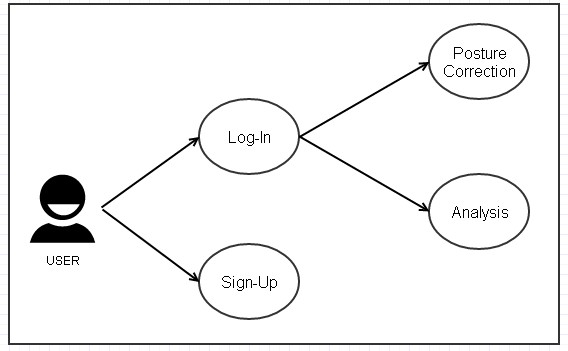
\includegraphics[scale=0.58]{img_17.jpg}
    \caption{Overall Usecase} 
\end{center}
\end{figure}

The overall usecase is shown in the Figure 16. Our project's platform is Android-Mobile Application. So, first user should download our application and execute the program to do self-orthotherapy. And if user executed the program, a dialog window to get permission of bluetooth and connect with Arduino would pop up. Then user will find the proper device and connect with the Arduino and finally could see the first page of our application. After that if user has registered already, user could enter into the next functions like 'Posture Correction' or 'Analysis'. If not, user should sign-up and register user's data into the program's database to use this program.   

\begin{figure}[H]
\begin{center}
    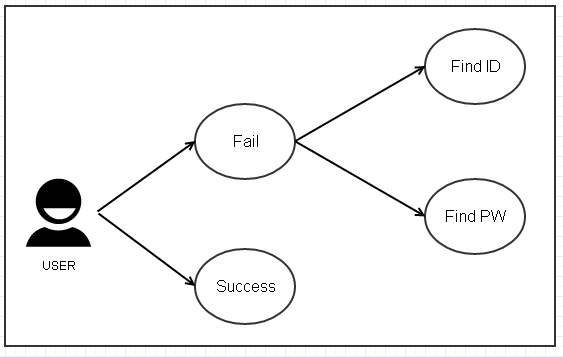
\includegraphics[scale=0.5]{img_18.png}
    \caption{Log-In Usecase} 
\end{center}
\end{figure}
 		
To use self-orthotherapy program, user should log-in to our system. But if user fails to do log-in, there are two ways of solving this problem. These are 'Find ID' and 'Find PW'. Log-In Usecase is shown in the Figure 17 and the Use Case's descriptions are written in the table 8.  




\begin{table}[h]
{\renewcommand\arraystretch{1.25}
\caption{The description of Log-In Usecase}
\begin{tabular}{|c|l|l|} \hline
Use Case & \multicolumn{2}{c|}{Description} \\ \hline\hline
Find ID& \multicolumn{2}{p{6.75cm}|}{\raggedright There are two ways to solve log-in problem. The first is 'Find ID'. User could find the own ID by writing the name and E-mail compared to the database's data.} \\ \hline
Find PW& \multicolumn{2}{p{6.75cm}|}{\raggedright And the second is 'Find PW'. User could find the own password by writing the ID, and name compared to the database's data. It could meet the need of 'Log-In' requirement.} \\ \hline
\end{tabular}}
\end{table}


\begin{figure}[H]
\begin{center}
    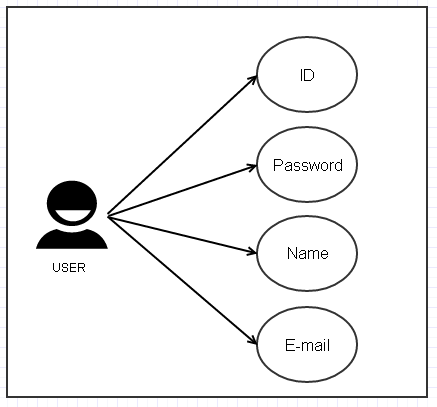
\includegraphics[scale=0.7]{img_19.png}
    \caption{Sign-up Usecase} 
\end{center}
\end{figure}
 		  
 
If user had not registered in our program, user should do sign-up to use the program. There are four componentes to register user's data into the database. It could meet the need of 'Sign-Up' requirement. Sign-Up Usecase is shown in the Figure 18 and the Use Case's descriptions are written in the table 9.

\begin{table}[h]
{\renewcommand\arraystretch{1.25}
\caption{The description of Sign-Up Usecase}
\begin{tabular}{|c|l|l|} \hline
Use Case & \multicolumn{2}{c|}{Description} \\ \hline\hline
ID& \multicolumn{2}{p{6.75cm}|}{\raggedright User should make unique ID to sign-up. It should be made of english and numbers under 10 characters. The special letters can not be used to make ID.And, it is mandatory for you to double-check your ID.} \\ \hline
Password & \multicolumn{2}{p{6.75cm}|}{\raggedright There is  no limit in the length of the password and the password will be replaced with other letters, such as ****, as soon as you enter your password for the sake of absolute confidentiality.} \\ \hline
Name& \multicolumn{2}{p{6.75cm}|}{\raggedright User should write own full name(first name + last name). And the english only could be used.} \\ \hline
E-mail& \multicolumn{2}{p{6.75cm}|}{\raggedright User should write one e-mail address. User could select the portal's address like 'gmail.com' or 'naver.com' or write the address in person. After that the permission e-mail will be sent to the written e-mail address. So, it is not possible to do sign-up unless the user do not check the permission e-mail.} \\ \hline
\end{tabular}}
\end{table} 

\begin{figure}[htbp]
\begin{center}
    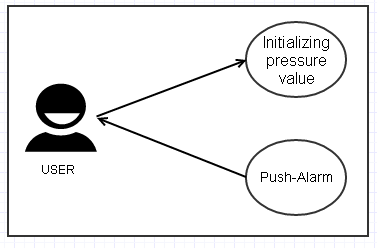
\includegraphics[scale=0.8]{img_20.png}
    \caption{Posture Correction Usecase} 
\end{center}
\end{figure}
 	  

The main function of this program is to correct user's bad posture when user sits down on the chair. So, setting the user's own pressure value is mendatory. Because people have different physical size and weight. Initializing pressure value  is the function to meet that requirement. After initializing pressure value, user could get alarm message when they keep bad posture. Posture Correction Usecase is shown in the Figure 19 and the Use Case's descriptions are written in the table 10.

\begin{table}[h]
{\renewcommand\arraystretch{1.25}
\caption{The description of Posture Correction Usecase}
\begin{tabular}{|c|l|l|} \hline
Use Case & \multicolumn{2}{c|}{Description} \\ \hline\hline
Initializing Pressure Value& \multicolumn{2}{p{4.5cm}|}{\raggedright To get posture correction alarm, initializing pressure value is needed. Because our algorithm needs the fixed pressure value suited to the user. So,  average of 5 times pressure values(when user sit down to the cushion, the pressure values are recognized.)is selected as the initial pressure value of user.} \\ \hline
Push-Alarm& \multicolumn{2}{p{4.5cm}|}{\raggedright If user has wrong posture, program would recognize that status using posture correction algorithm. And the push alarm will be popped up to the user's mobile phone like ''Do not make your leg crossed''.} \\ \hline
\end{tabular}}
\end{table}


\begin{figure}[H]
\begin{center}
    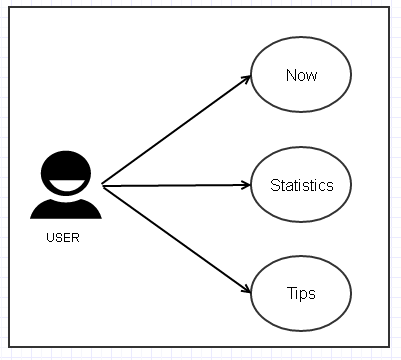
\includegraphics[scale=0.8]{img_21.png}
    \caption{Analysis Usecase} 
\end{center}
\end{figure}
               

 The another main function of this program is to offer analysis information using user's posture data. And there are three sub functions in analysis part 'Now', 'Statistics' and 'Tips'. Analysis Usecase is shown in the Figure 20 and the Use Case's descriptions are written in the table 11. 

\begin{table}[h]
{\renewcommand\arraystretch{1.25}
\caption{The description of Analysis Usecase}
\begin{tabular}{|c|l|l|} \hline
Use Case & \multicolumn{2}{c|}{Description} \\ \hline\hline
Now & \multicolumn{2}{p{6cm}|}{\raggedright User could see the two type of time in the 'Now' part. First is the the time of user's actual working hour. And the second is the time how much user keeps good posture and bad posture. And user could see the 3D feature reflecting user's present posture. So, it could help user recognize their present posture visually.} \\ \hline
Statistics & \multicolumn{2}{p{6cm}|}{\raggedright User could see the three type of analysing graphical data such as 'Day', 'Week' and 'Month'. The user's data is saved in the database and the program analyzes that data and shows the graphical graph using that data. So, user could see the data distribution according to the selected period(User could select period by touching the upper tab).  It meets the 'Statistics' and 'Visualization' requirements.} \\ \hline
Tips & \multicolumn{2}{p{6cm}|}{\raggedright User could see the some videos about stretching good for posture correction. And some of exercises which are good for posture correction  are recommended in this page.} \\ \hline
\end{tabular}}
\end{table}

\begin{figure}[H]
\begin{center}
    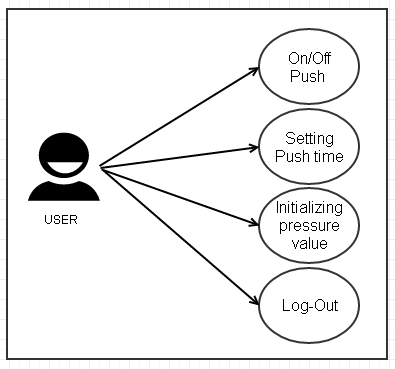
\includegraphics[scale=0.8]{img_22.png}
    \caption{Setting Usecase} 
\end{center}
\end{figure}
  	        	  

 User could do four functions in the Setting page. Those are 'On/Off Push', 'Setting Push time', 'Initializing pressure value' and 'Log-Out'. This functions could help user customize program's functions. Setting Usecase is shown in the Figure 21 and the Use Case's descriptions are written in the table 12.

\begin{table}[h]
{\renewcommand\arraystretch{1.25}
\caption{The description of Setting Usecase}
\begin{tabular}{|c|l|l|} \hline
Use Case & \multicolumn{2}{c|}{Description} \\ \hline\hline
On/Off Push & \multicolumn{2}{p{5cm}|}{\raggedright User could change the status of push alarm by On/Off. When user has urgent project meetint or needs to keep mobile phone silent, this function would be needed.} \\ \hline
Setting Push time & \multicolumn{2}{p{5cm}|}{\raggedright User could set the time when user get the push alarm. The time has range from 1 to 10 minutes. For example, if user selects 2 minutes in this page(Default value is 1 minute)user would get push alarm when user keeps bad posture for 2 minutes.  } \\ \hline
Initializing pressure value & \multicolumn{2}{p{5cm}|}{\raggedright User could intialize pressure value in this page. The reason why user uses this function is that the actual user could be changed. So, when the actual user is changed the program initializes the pressure value making average value getting five times pressure values. } \\ \hline
Log-Out & \multicolumn{2}{p{5cm}|}{\raggedright User could do Log-Out in this page. This function is required when user do not want to use this program or take out his/her own data to the database. } \\ \hline
\end{tabular}}
\end{table}



.\\\\\\\\\\\\\\\\\\\\\\\\\\\\\\\\\\\\\\\\\\\\\\\\\\\\\\\\\\\\\\\\\\\\\\\\\\\\\\\\\\\\\\\\\\\\\\\\\\\\\\\\\\\\\\\\\\\\\\\\\\\\\\\\\\

% An example of a floating figure using the graphicx package.
% Note that \label must occur AFTER (or within) \caption.
% For figures, \caption should occur after the \includegraphics.
% Note that IEEEtran v1.7 and later has special internal code that
% is designed to preserve the operation of \label within \caption
% even when the captionsoff option is in effect. However, because
% of issues like this, it may be the safest practice to put all your
% \label just after \caption rather than within \caption{}.
%
% Reminder: the "draftcls" or "draftclsnofoot", not "draft", class
% option should be used if it is desired that the figures are to be
% displayed while in draft mode.
%
%\begin{figure}[!t]
%\centering
%\includegraphics[width=2.5in]{myfigure}
% where an .eps filename suffix will be assumed under latex, 
% and a .pdf suffix will be assumed for pdflatex; or what has been declared
% via \DeclareGraphicsExtensions.
%\caption{Simulation Results}
%\label{fig_sim}
%\end{figure}

% Note that IEEE typically puts floats only at the top, even when this
% results in a large percentage of a column being occupied by floats.


% An example of a double column floating figure using two subfigures.
% (The subfig.sty package must be loaded for this to work.)
% The subfigure \label commands are set within each subfloat command, the
% \label for the overall figure must come after \caption.
% \hfil must be used as a separator to get equal spacing.
% The subfigure.sty package works much the same way, except \subfigure is
% used instead of \subfloat.
%
%\begin{figure*}[!t]
%\centerline{\subfloat[Case I]\includegraphics[width=2.5in]{subfigcase1}%
%\label{fig_first_case}}
%\hfil
%\subfloat[Case II]{\includegraphics[width=2.5in]{subfigcase2}%
%\label{fig_second_case}}}
%\caption{Simulation results}
%\label{fig_sim}
%\end{figure*}
%
% Note that often IEEE papers with subfigures do not employ subfigure
% captions (using the optional argument to \subfloat), but instead will
% reference/describe all of them (a), (b), etc., within the main caption.


% An example of a floating table. Note that, for IEEE style tables, the 
% \caption command should come BEFORE the table. Table text will default to
% \footnotesize as IEEE normally uses this smaller font for tables.
% The \label must come after \caption as always.
%
%\begin{table}[!t]
%% increase table row spacing, adjust to taste
%\renewcommand{\arraystretch}{1.3}
% if using array.sty, it might be a good idea to tweak the value of
% \extrarowheight as needed to properly center the text within the cells
%\caption{An Example of a Table}
%\label{table_example}
%\centering
%% Some packages, such as MDW tools, offer better commands for making tables
%% than the plain LaTeX2e tabular which is used here.
%\begin{tabular}{|c||c|}
%\hline
%One & Two\\
%\hline
%Three & Four\\
%\hline
%\end{tabular}
%\end{table}


% Note that IEEE does not put floats in the very first column - or typically
% anywhere on the first page for that matter. Also, in-text middle ("here")
% positioning is not used. Most IEEE journals/conferences use top floats
% exclusively. Note that, LaTeX2e, unlike IEEE journals/conferences, places
% footnotes above bottom floats. This can be corrected via the \fnbelowfloat
% command of the stfloats package.





% conference papers do not normally have an appendix


% use section* for acknowledgem



% trigger a \newpage just before the given reference
% number - used to balance the columns on the last page
% adjust value as needed - may need to be readjusted if
% the document is modified later
%\IEEEtriggeratref{8}
% The "triggered" command can be changed if desired:
%\IEEEtriggercmd{\enlargethispage{-5in}}

% references section

% can use a bibliography generated by BibTeX as a .bbl file
% BibTeX documentation can be easily obtained at:
% http://www.ctan.org/tex-archive/biblio/bibtex/contrib/doc/
% The IEEEtran BibTeX style support page is at:
% http://www.michaelshell.org/tex/ieeetran/bibtex/
%\bibliographystyle{IEEEtran}
% argument is your BibTeX string definitions and bibliography database(s)
%\bibliography{IEEEabrv,../bib/paper}
%
% <OR> manually copy in the resultant .bbl file
% set second argument of \begin to the number of references
% (used to reserve space for the reference number labels box)




% that's all folks
\end{document}
